\section{Introduction}

\textbf{Large Scale}
Problem of dimension $n$ but iterations $\ll n$ desired

\textbf{Convex}
One of the only problem classes that are \textquote{solvable}

\textbf{Optimization}
of objective function $f$ with decision variable $x$
considering feasible set $\mathcal{C} = \{\xi \in \mathbb{R}^{n}: g(\xi)\le0,\ h(\xi)=0\}$

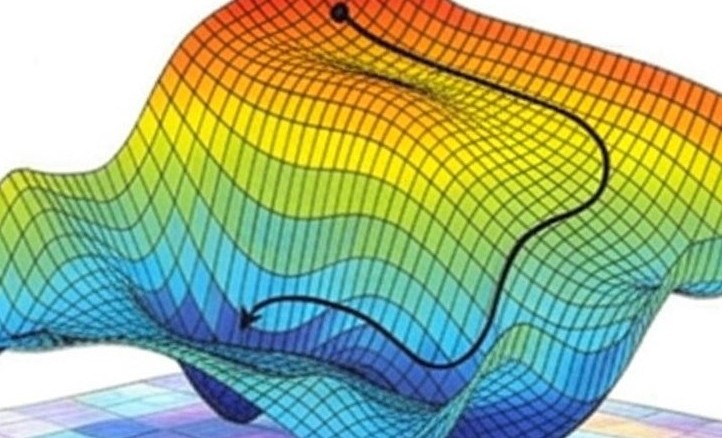
\includegraphics[width=\columnwidth]{images/head-image.jpg}
\textbf{Local minimum}
$x^\star$ if $\exists\epsilon>0$ s.t. $f(x^\star)\leq f(x)$,
$\forall x \in \mathcal{C} \cap B_\epsilon(x^\star)$,
$B_\epsilon(x^\star):=\{\xi\in\mathbb{R}^{n}:|\xi-x^\star|<\epsilon\}$


\begin{proposition}
	$f$ (lower-semi-)continuous,
	radially unbounded,
	% $|x|\rightarrow\infty\Rightarrow f(x)\rightarrow\infty$,
	$\mathcal{C}$ closed
	$\Rightarrow\exists$
	$	\min_{x \in \mathcal{C}} f(x)\ \text{and}\ x^\star\in\argmin_{x \in \mathcal{C}}f(x)$
\end{proposition}


\begin{definition}[Lipschitz continuity]
	$q: \mathbb{R}^{n} \rightarrow \mathbb{R}^{m}$
	is Lipschitz with constant $L$ if:
	$|q(x)-q(y)| \le L |x-y| \forall x,y \in \mathbb{R}^{m}$
\end{definition}
\vspace{-4mm}
$$f \text{ is\textbf{ Lipschitz }(Lip) with constant } L
	\Leftrightarrow
	|\nabla f(x)|_2\le L$$
\vspace{-4mm}

OP class $\mathcal{P}$ with $\mathcal{C}=[0,1]^n$,
$f$ is $l^\infty$-Lipschitz with constant $L$

\begin{proposition}
	For any algorithm $\exists$ problem in $\mathcal{P}$,
	s.t. achieving $|f(x_N )−f(x^⋆)| < \epsilon$
	requires
	$N \ge (\lfloor\frac{L}{2\epsilon}\rfloor)^n-1$
\end{proposition}

\begin{definition}
	OP convex if, $f$ and $g_i$ convex functions, $h$ affine.
\end{definition}


\begin{definition}
	$q:\mathbb{R}^{n}\rightarrow\mathbb{R}$
	convex (affine) if $\forall\ x, y \in \mathbb{R}^{n}$
	\vspace{-1mm}
	$$q(\theta x+(1−\theta)y)\le\theta q(x)+(1−\theta)q(y)\quad\forall\ \theta \in [0, 1]$$
	\vspace{-3mm}
\end{definition}
\vspace{-1mm}
\begin{proposition}
	OP convex
	$\Rightarrow$
	local minimum $=$ global minimum
\end{proposition}


